\documentclass{article}
\usepackage[utf8]{inputenc}
\usepackage[spanish]{babel}
\usepackage{listings}
\usepackage{graphicx}
\graphicspath{ {images/} }
\usepackage{cite}
\usepackage{amssymb, amsmath}

\begin{document}

\begin{titlepage}
    \begin{center}
        \vspace*{1cm}
            
        \Huge
        \textbf{Parcial 1: Informática II}
            
        \vspace{0.5cm}
        \LARGE
       Análisis y diseño.
          
            
        \vspace{5cm}
            
        \textbf{
        JOSE MIGUEL GOMEZ MONSALVE
        ERIKA LEÓN QUIROGA\newline
        DAVID AGUDELO OCHOA
        }
        
        
        
            
        \vfill
            
        \vspace{0.8cm}
       
        \Large


        \vfill
        Despartamento de Ingeniería Electrónica y Telecomunicaciones\\
        Universidad de Antioquia\\
        Medellín\\
        Febrero 2022
                 
    \end{center}
\end{titlepage}

\tableofcontents\newpage
\section{Introducción}
\noindent

\newpage

\section{Integrado 74HC595.} \label{Integrado}
El integrago 74HC595 hace parte de la familia de dispositivos SNx4HC59, la cual contienen un registro de desplazamiento de 8 bits de entrada en serie y salida en paralelo, el registro de almacenamiento tiene salidas de 3 estados paralelos. Se proporcionan relojes separados para el registro de desplazamiento y el de almacenamiento. El registro de desplazamiento tiene una entrada de anulación directa (SRCLR), una entrada en serie (SER) y salidas en serie para la conexión en cascada. Tienen una amplia corriente de funcionamiento de 2 V a 6 V, y las salidas de 3 estados de alta corriente pueden controlar hasta 15 cargas LSTTL. Los dispositivos tienen un bajo consumo consumo de 80-μA (máximo) ICC.
\subsection{Características del integrado.}\label{caracteristicas}
 \begin{itemize}
 
\item Entrada serial, salida paralela, o salida serial que permite la conexión en cascada de varios integrados.
\item Registro de desplazamiento de 8 bits que alimenta a un registro de almacenamiento.
\item Entradas de reloj separadas para el registro de desplazamiento y el de almacenamiento con activación por flanco de subida.

\end{itemize}

\begin{figure}[h]
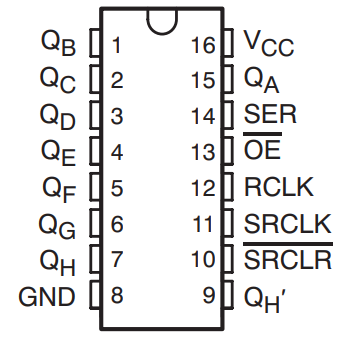
\includegraphics[scale=1]{esquematico.png}
\centering
\caption{Integrado 74HC595.}
\label{fig:func1}
\end{figure}

\textbf{Configuración de pines.}
\newline
\begin{itemize}
\item Los pines de $Q_B$(pin 1) a $Q_H$(pin 7), añadiendo $Q_A$(pin 15) representan las salidas del integrado.
\item $V_C_C$(pin 16) es la alimentación y GND(pin 8) se conecta a tierra.
\item $Q_H_'$(pin 9) se utiliza para conectar otro integrado 74HC595 y generar un efecto de cascada.
\item El pin 14 o SER es el pin donde se envían los datos.
\item $\Bar{OE}$(pin 13) llamado Output Enable, habilita las salidas y se activa con un nivel bajo, por lo cual, para que siempre esté activo se conecta a GND.
\item El RCLK (pin 12) es el reloj del registro de almacenamiento y se utiliza para actualizar los datos a los pines de salida.
\item El SRCLK (pin 11) es el reloj que sincroniza la carga de datos.
\item El $\Bar{SRCLR}$ (pin 11) llamado Shift Register Clear, reestablece el registro de desplazamiento.


\end{itemize}

\subsection{Funcionamiento.}\label{integrado funcionamiento}


\begin{figure}[h]
\includegraphics[scale=0.8]{funcionamiento1.png}
\centering
\caption{Iniciar el programa.}
\label{fig:func1}
\end{figure}


\subsection{Aplicaciones.}\label{Aplicaciones}
\begin{itemize}
\item Network switches
\item Power infrastructure
\item LED displays
\item Servers
\end{itemize}

\end{document}
